\documentclass[a4paper]{tufte-book}
\raggedbottom

%----------%
% SETTINGS %
%----------%

\makeatletter
\def\input@path{{./settings/}}
\makeatother
\usepackage{lipsum}
\usepackage{hyperref}
\usepackage{import}  % for relative paths importing

% Packages
\usepackage{amsmath, mathtools, bm, commath}
\usepackage{physics}
\usepackage{siunitx}
\usepackage{nicematrix}

% General settings
\allowdisplaybreaks     % Allows for equations to break between pages

% Cancel-lines related
\usepackage[thicklines]{cancel}
\renewcommand\CancelColor{\color{xred}}
\newcommand{\cancelcol}[2][xred]{ % This is such a silly solution...
	\renewcommand\CancelColor{\color{#1}}
	\cancel{#2}
	\renewcommand\CancelColor{\color{xred}}
}

% Easier space-notation
\newcommand{\Rs}[1][]{\mathbb{R}^{#1}}
\newcommand{\Cs}[1][]{\mathbb{C}^{#1}}

% Set notation for vectors (currently: bold letters)
\renewcommand{\vec}[1]{\bm{#1}}
\newcommand{\uvec}[1]{\bm{\hat{#1}}}
\newcommand{\vnorm}[1]{\left\| \vec{#1} \right\|}
\newcommand{\cvec}[1]{\bm{\overline{#1}}}
\newcommand{\mat}[1]{\bm{#1}}

% Identity matrix
\newcommand{\Id}[1]{\mathbb{I}_{#1}}

% Vector operations
\newcommand{\inner}[2]{\langle #1,#2 \rangle}

% Dual space related
\newcommand{\dualspace}[1]{#1^{*}}
\newcommand{\dualvec}[1]{\vec{#1}^{*}}
\newcommand{\dualbasis}[1]{#1^{*}}
\newcommand{\dualeb}[1]{\dualvec{e}_{#1}}
\newcommand{\dualRs}[1][]{\mathbb{R}^{#1*}}
\newcommand{\dualCs}[1][]{\mathbb{C}^{#1*}}

% Row- and column-vectors: arguments separated by ";".
% Example: $\vec{a} = \colvec{1;2;3;4}$.
\makeatletter
\newcommand\rcvector[2][\\]{\ensuremath{%
  \global\def\rc@delim{#1}%
    \negthinspace\begin{bmatrix}
      \rc@vector #2;\relax\noexpand\@eolst%
    \end{bmatrix}}}
\def\rc@vector #1;#2\@eolst{%
  \ifx\relax#2\relax
    #1
  \else
    #1\rc@delim
    \rc@vector #2\@eolst%
  \fi}
\makeatother
\newcommand{\colvec}{\rcvector}
\newcommand{\rowvec}[1]{\rcvector[,\;]{#1}}
\newcommand{\GenericRowVec}[2][n]{\rowvec{#2_{1};#2_{2};\dots;#2_{#1}}}
\newcommand{\GenericColVec}[2][n]{\colvec{#2^{1};#2^{2};\vdots;#2^{#1}}}

% Colored vectors
\newcommand{\colorVec}[2]{\color{#1}{\vec{#2}}\color{black}}
\newcommand{\vred}{\colorVec{xdarkred}{v}}
\newcommand{\vblue}{\colorVec{xdarkblue}{v}}
\newcommand{\vgreen}{\colorVec{xdarkgreen}{v}}

% Basis vectors and transformations
\newcommand{\eb}[1]{\vec{e}_{#1}}
\newcommand{\ebc}[1]{\tilde{\vec{e}}_{#1}}
\newcommand{\ebr}[1]{\color{xdarkblue}\eb{#1}\color{black}}
\newcommand{\ebcr}[1]{\color{xdarkred}\ebc{#1}\color{black}}
\newcommand{\oldB}{\color{xdarkblue}B\color{black}}
\newcommand{\newB}{\color{xdarkred}\tilde{B}\color{black}}
\newcommand{\Forw}{\bm{F}}
\newcommand{\Backw}{\bm{F^{-1}}}

% Dark equal?
\newcommand{\beq}{\color{black}{=}}

% Better imaginary unit and natural base notation (to separate from variables)
\newcommand{\iu}{\mathrm{i}\mkern1mu}
\newcommand{\eu}{\mathrm{e}}
\newcommand{\Eu}[1]{\mathrm{e}^{#1}}
\newcommand{\EX}[1]{\exp\left(#1\right)}

% General nice matrix
\newcommand{\GNMatrix}[3]{
  \begin{bNiceMatrix}
    #1_{11} & #1_{12} & \dots & #1_{1#3}\\
    #1_{21} & #1_{22} & \dots & #1_{2#3}\\
    \vdots & \vdots & \Ddots & \vdots\\
    #1_{#21} & #1_{#22} & \dots & #1_{#2#3}
  \end{bNiceMatrix}
}

% Clever references (tufte-latex clashes with \autoref)
\usepackage{cleveref}
\crefname{figure}{Figure}{Figure}

% Hyperrefs etc.
\usepackage{hyperref}
\hypersetup{
  colorlinks=true,
  linkcolor=blue,
  filecolor=magenta,      
  urlcolor=cyan,
  pdftitle={Spinors for Beginners},
  pdfauthor={Peleg Bar Sapir},
}

% Packages
\usepackage{xcolor}

%%%%%%%%%%%%%%%%%%%%%%%%
%        COLORS        %
%%%%%%%%%%%%%%%%%%%%%%%%

% Normal colors
\definecolor{xred}{HTML}{BD4242}
\definecolor{xblue}{HTML}{4268BD}
\definecolor{xgreen}{HTML}{52B256}
\definecolor{xpurple}{HTML}{7F52B2}
\definecolor{xorange}{HTML}{FD9337}
\definecolor{xdotted}{HTML}{999999}
\definecolor{xgray}{HTML}{777777}
\definecolor{xcyan}{HTML}{80F5DC}
\definecolor{xpink}{HTML}{F690EA}
\definecolor{xgrayblue}{HTML}{49B095}
\definecolor{xgraycyan}{HTML}{5AA1B9}

% Dark colors
\colorlet{xdarkred}{red!85!black}
\colorlet{xdarkblue}{xblue!85!black}
\colorlet{xdarkgreen}{xgreen!85!black}
\colorlet{xdarkpurple}{xpurple!85!black}
\colorlet{xdarkorange}{xorange!85!black}
\colorlet{xdarkcyan}{xcyan!85!black}

% Very dark colors
\colorlet{xverydarkblue}{xblue!50!black}

% Document-specific colors
\colorlet{normaltextcolor}{black}
\colorlet{figtextcolor}{xblue}

% Enumerated colors
\colorlet{xcol0}{black}
\colorlet{xcol1}{xred}
\colorlet{xcol2}{xblue}
\colorlet{xcol3}{xgreen}
\colorlet{xcol4}{xpurple}
\colorlet{xcol5}{xorange}
\colorlet{xcol6}{xcyan}
\colorlet{xcol7}{xpink!75!black}

%%%%%%%%%%%%%%%%%%%%%
%        PGF        %
%%%%%%%%%%%%%%%%%%%%%

\usepackage{pgfplots}
\usepgfplotslibrary{fillbetween}%, colormaps, colorbrewer, patchplots}
\pgfplotsset{
  compat=1.16,
  %% Styles %%
  xyplane/.style = {
    axis x line=middle,
    axis y line=middle,
    xlabel=$x$,
    ylabel=$y$,
    every axis x label/.style={at={(ticklabel* cs:1.02)}, anchor=west},
    every axis y label/.style={at={(ticklabel* cs:1.02)}, anchor=south},
    axis line style={stealth-stealth, very thick, black!65},
    label style={font=\large},
    tick label style={font=\large},
    samples=100,
    xmin=-5, xmax=5,
    ymin=-5, ymax=5,
    grid=both,
    major grid style={black!15},
    minor grid style={black!10},
    xticklabels={,},
    yticklabels={,},
  },
  xynogrid/.style = {
    xyplane,
    major grid style={opacity=0},
    minor grid style={opacity=0},
  },
  xyempty/.style = {
    xyplane,
    axis line style = {draw=none},
    tick style = {draw=none},
    xlabel = {},
    ylabel = {},
    major grid style = {draw=black!0},
  },
  hyperplane1D/.style = {thick, #1},
  %% Function plots
  function/.style = {
    ultra thick, draw=#1,
  },
  filledfunction/.style = {
    function={#1}, opacity=1, fill=#1, fill opacity=0.3,
  },
}

%%%%%%%%%%%%%%%%%%%%%%
%        TikZ        %
%%%%%%%%%%%%%%%%%%%%%%

\usepackage{tikz, tikz-3dplot}
\usetikzlibrary{calc, shapes, intersections, backgrounds}
\tikzset{
  %% Styles %%
  vector/.style = {#1, ultra thick, -stealth, cap=round},
  pics/ruler/.style n args = {5}{
      code = {
          % Parameters
          \pgfmathsetmacro{\width}{#1}
          \pgfmathsetmacro{\height}{#2}
          \pgfmathsetmacro{\yMaj}{\height/3}
          \pgfmathsetmacro{\yMid}{\yMaj*0.7}
          \pgfmathsetmacro{\yMin}{\yMaj*0.5}
          \pgfmathsetmacro{\dxMaj}{#3}
          \pgfmathsetmacro{\dxMin}{\dxMaj*0.1}
          \pgfmathsetmacro{\maxMajGrad}{ceil((\width-2)/\dxMaj)}
          \pgfmathsetmacro{\maxMidGrad}{\maxMajGrad-0.5}
          \pgfmathsetmacro{\maxMinGrad}{(\maxMajGrad-1)*10}

          % Main rectangle
          \draw[thick, fill=#4] (0,0) rectangle (\width,\height);

          % Graduations
          % Major
          \foreach \x [count=\k from 0] in {1,2,...,\maxMajGrad}
              \draw[thick] ({\x*\dxMaj}, \height) -- ++(0.0,-\yMaj) node[below] (g\k) {$\k$};
          % Middle
          \foreach \y in {1.5,2.5,...,\maxMidGrad}
              \draw[thick] ({\y*\dxMaj}, \height) -- ++(0.0,-\yMid);
          % Minor
          \foreach \z in {1,2,...,\maxMinGrad} 
              \draw[thin] ({\dxMaj+\z*\dxMin}, \height) -- ++(0.0,-\yMin);

          % units label
          \node[below of=g0, font=\small, yshift={11*\height}] {#5};
      }
  }
}
\newcommand{\rulerTwoD}[6]{
  \pgfmathsetmacro{\Vx}{#1};
  \pgfmathsetmacro{\Vy}{#2};
  \pgfmathsetmacro{\a}{#3};
  \pgfmathsetmacro{\scale}{3*\a/sqrt(\Vx*\Vx+\Vy*\Vy)};
  \foreach \b in {-#4,...,#4}
    \addplot[very thick, #5] {-(\Vx/\Vy)*x+(\b/\a)};
}

% section numbering
\setcounter{secnumdepth}{2}

% Chapter title
\titleformat{\chapter}
[block]% shape
{\relax\ifthenelse{\NOT\boolean{@tufte@symmetric}}{\begin{fullwidth}}{}}% format applied to label+text
{\itshape\huge\thechapter}% label
{1em}% horizontal separation between label and title body
{\huge\rmfamily\itshape}% before the title body
[\ifthenelse{\NOT\boolean{@tufte@symmetric}}{\end{fullwidth}}{}]% after the title body


%----------%
% DOCUMENT %
%----------%

\begin{document}
% \part{Tests}
% \chapter{General layout test}
% \section{This is a title}\label{sec:title}
\lipsum[2-2]

\begin{marginfigure}
    \begin{center}
    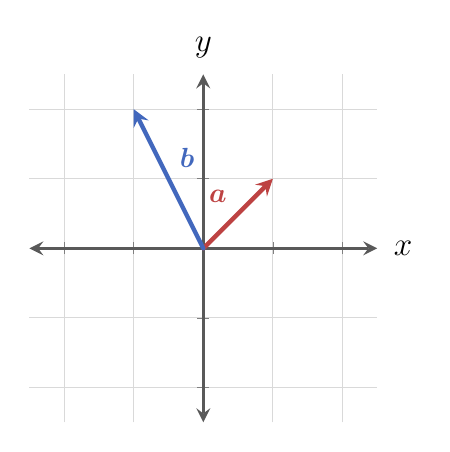
\begin{tikzpicture}
    \begin{axis}[
        xyplane,
        width=6cm, height=6cm,
    ]
        \draw[vector={xred}] (0,0) -- (2,2) node[midway, above left] {$\vec{a}$};
        \draw[vector={xblue}] (0,0) -- (-2,4) node[midway, above right] {$\vec{b}$};
    \end{axis}
    \end{tikzpicture}
    \end{center}
    \caption{A margin figure.}
    \label{fig:margin_figure}
\end{marginfigure}

This is a manualy-typed text. It even points to a figure (see \autoref{fig:margin_figure}).


\makeatletter

%% -- PART 1: Background -- %%
\part{Background Topics}

% Linear algebra
\chapter{Linear Algebra}
\def\input@path{{./parts/background/linear_algebra}}
\section{Preface}
\newthought{The goal of this chapter} is not to teach you, the reader, linear algebra from scratch - nor to be a thorough source of information on the topic. Rather, my aim is to overview the topic in such a way that new-comers, as well as those who studied linear algebra in an undergraduate university course, will gain the important insights of the topic needed for understanding the rest of the background material and spinors as well.

Instead of teaching the topic from the ground-up, like mathematicians tend to do\sidenote{In my view, courses that \enquote{build} linear algebra step-by-step give the students good knowledge of the structures of vector spaces, but tend to miss the intuitive view of what these structures can \textit{do}. This is exactly the difference between the \enquote{pure} mathematics of the mathematician and the mathematics as a tool of the scientist.}, I prefer to stick to the geometric interpretation of the vector spaces $\Rs[2]$ and $\Rs[3]$ (and to a lesser extent $\Rs[n]$ in general). These interpretations can be visualized relatively easily, and thus help in setting up the needed intuition in the student's mind, which becomes handy when the topic turns to more abstract constructs (such as for example vector spaces of matrices or functions).

In my personal experiences, when I was studying the topic I completely failed to understand it (and indeed, failed the courses I took) until it \enquote{clicked} for me in regards to 2- and 3-dimensional real spaces, i.e. - visible geometry. Then I didn't even have to study for exams anymore, as everything became clear enough to grasp and develop on the spot even during an exam (except for later, more advances concepts). That is why, for example, I absolutely adore courses and study materials of the topic\sidenote{And other mathematical topics as well.} which use animation, such as \textit{3Blue1Brown} great video essay series \href{https://www.3blue1brown.com/topics/linear-algebra}{Essence of linear algebra}\sidenote{Temporary sidenote which should become a citation for the mentioned 3B1B video series}.

There are very few proofs in this chapter, and those that are shown are not completely rigorous. For more in-depth materials, see the last section (further read). With that out of the way - let's begin!
\newpage

\section{Vectors and Vector Spaces}
\newthought{Vectors are }the most basic and important element in linear algebra. There are several different approaches to defining a vector: physicists like to talk about vectors as objects with magnitude and direction. Computer scientists and programmers tend to view vectors as lists of numbers (and sometimes other types of objects as well). To the mathematician, vectors are elements of \textit{vector sets}, which are defined rigorously and precisely.

The existence of different definitions leads to much confusion\sidenote{I admit that this is a classic case of \enquote{citation needed}, but it is something I come across often.}: for example, we usually think of matrices as \textit{acting} on vectors, so how can matrices be vectors themselves? Also - are vectors just list of numbers, or are there some such lists that aren't vectors? Can we always reduce any vector to a list of numbers? And what about the case of functions as vectors? Etc., etc.

Therefore, for now I choose to limit the definition of vectors to the so-called \enquote{physicist's definition}: a vector is an object which has both a magnitude (also \textit{length} and \textit{norm}), and a direction. These can be easily visualized in 2- and 3-dimensional real spaces as arrows. We will later see how this translates into lists of numbers (and later still how we can define more abstract and inclusive vectors). Since vectors don't have positions, we can freely move them around in space, and normally present them as originating from the same point in space (\cref{fig:vectors}).

\begin{marginfigure}
    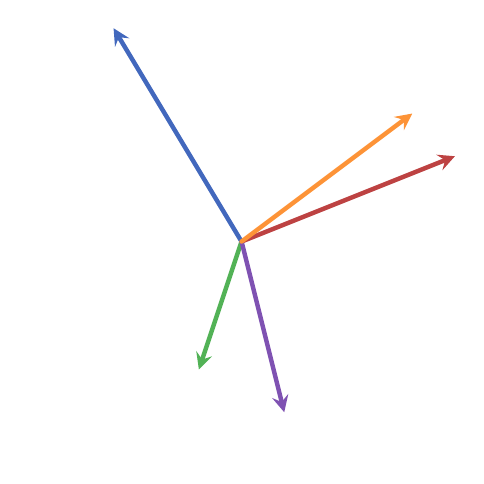
\begin{tikzpicture}
    \begin{axis}[
        xyempty,
        width=7cm, height=7cm,
        ]
        \draw[vector={xred}] (0,0) -- (5,2);
        \draw[vector={xblue}] (0,0) -- (-3,5);
        \draw[vector={xgreen}] (0,0) -- (-1,-3);
        \draw[vector={xpurple}] (0,0) -- (1,-4);
        \draw[vector={xorange}] (0,0) -- (4,3);
    \end{axis}
    \end{tikzpicture}
    \caption{Some vectors placed in 2-dimensional space such that they all originate from the same point.}
    \label{fig:vectors}
\end{marginfigure}

Let's now overview the basic operations that can be done with vectors. One operation is \textit{scaling} by a real number: scaling a vector means that we're changing the norm of the vector without changing its direction (\cref{fig:scaling_vectors}). Note that by direction we mean the line going through the vector's origin and its head: when we scale a vector by a negative number $\alpha\in\Rs$ we flip the vector's orientation and scale its norm by the absolute value of $\alpha$ - the vector is then considered to stay in the same direction in space (\cref{fig:scaling_vectors}, again). Generally, the norm of a vector $\vec{u}$ is denoted using double vertical lines: $\vnorm{u}$.

\begin{marginfigure}
    \resizebox{4cm}{!}{
        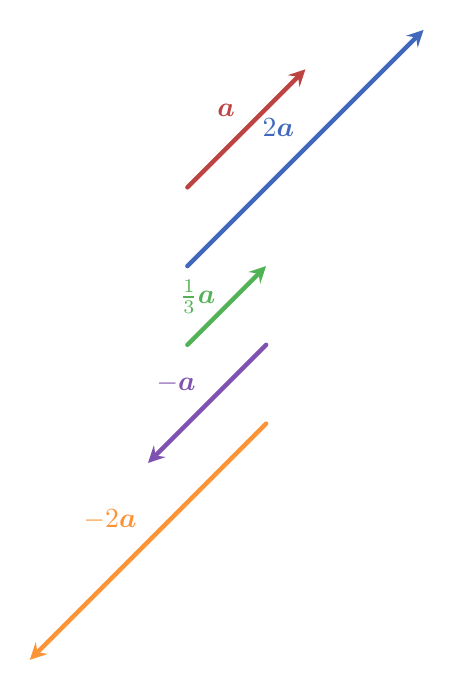
\begin{tikzpicture}
            \draw[vector={xred}] (0,0) -- ++(1.5,1.5) node[midway, above left] {$\vec{a}$};
            \draw[vector={xblue}] (0,-1) -- ++(3,3) node[midway, above left] {$2\vec{a}$};
            \draw[vector={xgreen}] (0,-2) -- ++(1,1) node[midway, above left, yshift=-7pt] {$\frac{1}{3}\vec{a}$};
            \draw[vector={xpurple}] (1,-2) -- ++(-1.5,-1.5) node[midway, above left] {$-\vec{a}$};
            \draw[vector={xorange}] (1,-3) -- ++(-3,-3) node[midway, above left] {$-2\vec{a}$};
        \end{tikzpicture}
    }
    \caption{Some vectors placed in the origin of a 2-dimensional Cartesian coordinate system.}
    \label{fig:scaling_vectors}
\end{marginfigure}

A vector which has norm of $1$ is called a \textit{unit vector}. We will denote unit vectors in the book using the regular bold notation with a \enquote{hat} on top of it: $\uvec{a}$. Any vector can be made into a unit vector (be \textit{normalized}) by scaling the vector by the reciprocal of its norm (if it isn't zero): given a vector $\vec{u}$, we can scale it by $\vnorm{u}^{-1}$ and get the unit vector $\uvec{u}$, i.e.
\begin{equation}
    \uvec{u} = \frac{1}{\vnorm{u}}\vec{u}.
    \label{eq:label}
\end{equation}

Vectors can also be added together using the \textit{parallelogram rule}: given two vectors $\vec{a}$ and $\vec{b}$ we first place $\vec{b}$ such that its origin lies on the head of $\vec{a}$. The vector $\vec{c}$ from the origin of $\vec{a}$ to the head of $\vec{b}$ is the result of the addition.

\section{Linear Transformations}

\section{Matrices}

\section{Eigenvectors and Eigenvalues}

\section{Quaternions and Octanions}

\section{Advanced Notation and Einstein's Summation}

\section{Further Reading}


% - Geometric algebra
\chapter{Geometric Algebra}
\def\input@path{{./parts/background/geometric_algebra}}
\section{Preface}
\newthought{The goal of this chapter} is not to teach you, the reader, linear algebra from scratch - nor to be a thorough source of information on the topic. Rather, my aim is to overview the topic in such a way that new-comers, as well as those who studied linear algebra in an undergraduate university course, will gain the important insights of the topic needed for understanding the rest of the background material and spinors as well.

Instead of teaching the topic from the ground-up, like mathematicians tend to do\sidenote{In my view, courses that \enquote{build} linear algebra step-by-step give the students good knowledge of the structures of vector spaces, but tend to miss the intuitive view of what these structures can \textit{do}. This is exactly the difference between the \enquote{pure} mathematics of the mathematician and the mathematics as a tool of the scientist.}, I prefer to stick to the geometric interpretation of the vector spaces $\Rs[2]$ and $\Rs[3]$ (and to a lesser extent $\Rs[n]$ in general). These interpretations can be visualized relatively easily, and thus help in setting up the needed intuition in the student's mind, which becomes handy when the topic turns to more abstract constructs (such as for example vector spaces of matrices or functions).

In my personal experiences, when I was studying the topic I completely failed to understand it (and indeed, failed the courses I took) until it \enquote{clicked} for me in regards to 2- and 3-dimensional real spaces, i.e. - visible geometry. Then I didn't even have to study for exams anymore, as everything became clear enough to grasp and develop on the spot even during an exam (except for later, more advances concepts). That is why, for example, I absolutely adore courses and study materials of the topic\sidenote{And other mathematical topics as well.} which use animation, such as \textit{3Blue1Brown} great video essay series \href{https://www.3blue1brown.com/topics/linear-algebra}{Essence of linear algebra}\sidenote{Temporary sidenote which should become a citation for the mentioned 3B1B video series}.

There are very few proofs in this chapter, and those that are shown are not completely rigorous. For more in-depth materials, see the last section (further read). With that out of the way - let's begin!
\newpage


% - Abstract algebra
\chapter{Abstract Algebra}
\def\input@path{{./parts/background/abstract_algebra}}
\section{Preface}
\newthought{The goal of this chapter} is not to teach you, the reader, linear algebra from scratch - nor to be a thorough source of information on the topic. Rather, my aim is to overview the topic in such a way that new-comers, as well as those who studied linear algebra in an undergraduate university course, will gain the important insights of the topic needed for understanding the rest of the background material and spinors as well.

Instead of teaching the topic from the ground-up, like mathematicians tend to do\sidenote{In my view, courses that \enquote{build} linear algebra step-by-step give the students good knowledge of the structures of vector spaces, but tend to miss the intuitive view of what these structures can \textit{do}. This is exactly the difference between the \enquote{pure} mathematics of the mathematician and the mathematics as a tool of the scientist.}, I prefer to stick to the geometric interpretation of the vector spaces $\Rs[2]$ and $\Rs[3]$ (and to a lesser extent $\Rs[n]$ in general). These interpretations can be visualized relatively easily, and thus help in setting up the needed intuition in the student's mind, which becomes handy when the topic turns to more abstract constructs (such as for example vector spaces of matrices or functions).

In my personal experiences, when I was studying the topic I completely failed to understand it (and indeed, failed the courses I took) until it \enquote{clicked} for me in regards to 2- and 3-dimensional real spaces, i.e. - visible geometry. Then I didn't even have to study for exams anymore, as everything became clear enough to grasp and develop on the spot even during an exam (except for later, more advances concepts). That is why, for example, I absolutely adore courses and study materials of the topic\sidenote{And other mathematical topics as well.} which use animation, such as \textit{3Blue1Brown} great video essay series \href{https://www.3blue1brown.com/topics/linear-algebra}{Essence of linear algebra}\sidenote{Temporary sidenote which should become a citation for the mentioned 3B1B video series}.

There are very few proofs in this chapter, and those that are shown are not completely rigorous. For more in-depth materials, see the last section (further read). With that out of the way - let's begin!
\newpage


% - Lie groups and algebras
\chapter{Lie Groups and Algebras}
\def\input@path{{./parts/background/lie_groups_algebras}}
\section{Preface}
\newthought{The goal of this chapter} is not to teach you, the reader, linear algebra from scratch - nor to be a thorough source of information on the topic. Rather, my aim is to overview the topic in such a way that new-comers, as well as those who studied linear algebra in an undergraduate university course, will gain the important insights of the topic needed for understanding the rest of the background material and spinors as well.

Instead of teaching the topic from the ground-up, like mathematicians tend to do\sidenote{In my view, courses that \enquote{build} linear algebra step-by-step give the students good knowledge of the structures of vector spaces, but tend to miss the intuitive view of what these structures can \textit{do}. This is exactly the difference between the \enquote{pure} mathematics of the mathematician and the mathematics as a tool of the scientist.}, I prefer to stick to the geometric interpretation of the vector spaces $\Rs[2]$ and $\Rs[3]$ (and to a lesser extent $\Rs[n]$ in general). These interpretations can be visualized relatively easily, and thus help in setting up the needed intuition in the student's mind, which becomes handy when the topic turns to more abstract constructs (such as for example vector spaces of matrices or functions).

In my personal experiences, when I was studying the topic I completely failed to understand it (and indeed, failed the courses I took) until it \enquote{clicked} for me in regards to 2- and 3-dimensional real spaces, i.e. - visible geometry. Then I didn't even have to study for exams anymore, as everything became clear enough to grasp and develop on the spot even during an exam (except for later, more advances concepts). That is why, for example, I absolutely adore courses and study materials of the topic\sidenote{And other mathematical topics as well.} which use animation, such as \textit{3Blue1Brown} great video essay series \href{https://www.3blue1brown.com/topics/linear-algebra}{Essence of linear algebra}\sidenote{Temporary sidenote which should become a citation for the mentioned 3B1B video series}.

There are very few proofs in this chapter, and those that are shown are not completely rigorous. For more in-depth materials, see the last section (further read). With that out of the way - let's begin!
\newpage


%% -- PART 2: Spinors -- %%
\part{Spinors}


\makeatother
\end{document}
